% !TEX root = ../FCT_radiation_paper.tex

This section presents results for a number of test problems, which compare
the solutions obtained using:
\begin{itemize}
  \item the standard Galerkin FEM, labelled as ``Galerkin'' in the plots,
  \item the low-order method, labelled in plots as ``Low'',
  \item the entropy viscosity method, labelled in plots as ``EV'',
  \item the standard Galerkin FEM with FCT, labelled in plots as ``Galerkin-FCT'', and
  \item the entropy viscosity method with FCT, labelled in plots as ``EV-FCT''.
\end{itemize}
All problems assume a speed of $v=1$ (the speed effectively just changes the
units of $\dt$) and an entropy function of $\eta(u)=\frac{1}{2}u^2$. Unless
otherwise specified, the transport direction is in the positive
$x$ direction: $\mathbf{\Omega}=\mathbf{e}_x$, and the entropy
viscosity tuning parameters of $c_\mathcal{R}$ and $c_\mathcal{J}$ are set
to 0.1.

%===============================================================================
\subsection{Spatial Convergence Tests}
%===============================================================================
This 1-D, steady-state test problem uses the Method of Manufactured Solutions (MMS) with
a solution of $u(x)=\sin(\pi x)$ on the domain $x\in(0,1)$. Zero Dirichlet
boundary conditions are imposed on both boundaries.
With $\sigma(x)=1$,
the MMS source becomes $q(x)=\pi\cos(\pi x) + \sin(\pi x)$.
The number of cells in the study starts at 8 for the coarsest mesh, and cells
are refined by a factor of 2 in each cycle, ending with 256 cells.

Figure \ref{fig:mms_sinx_ss} shows the $L^2$ norm errors for this convergence study
and indicates first-order spatial convergence for the low-order method and
second-order spatial convergence for the entropy viscosity (EV) method
and EV-FCT method, as expected.
\begin{figure}[htb]
   \centering
      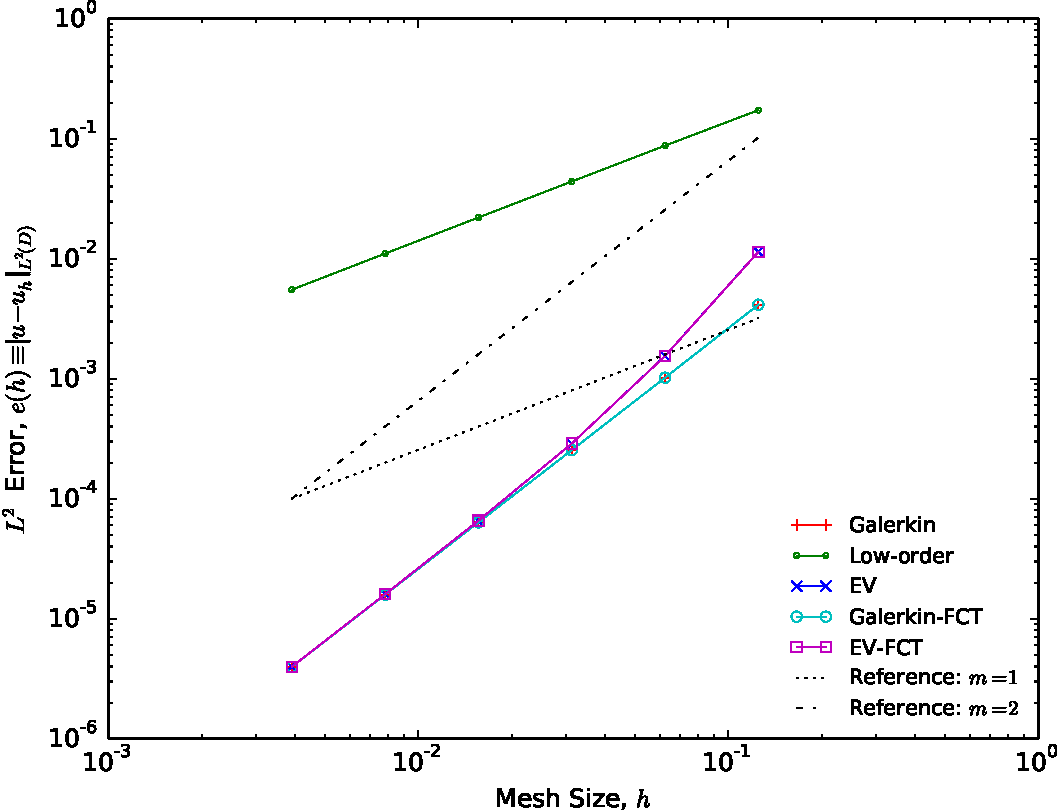
\includegraphics[width=\textwidth]
        {images/convergence_sinx.pdf}
      \caption{Spatial Convergence for MMS Problem}
   \label{fig:mms_sinx_ss}
\end{figure}
\clearpage
%===============================================================================
\subsection{Glancing Beam in a Void}
%===============================================================================
This 2-D test problem is on the unit square: $\x\in(0,1)^2$ and simulates
a beam incident on the bottom boundary of a void region
($\sigma(\x)= 0$, $q(\x)=0$) at a shallow angle of
$21.94^\circ$ with respect to the x-axis ($\Omega_x=\cos(21.94^\circ)$,
$\Omega_y=\sin(21.94^\circ)$).
The exact solution of this problem contains a discontinuity along the line
$y = \frac{\Omega_y}{\Omega_x}x$, which presents opportunity for the formation
of spurious oscillations.
This is run as a pseudo-transient problem with zero initial conditions until
steady-state is reached. A Dirichlet
boundary condition is imposed on the incoming sides of the problem, with a value of 1
on the bottom boundary and a value of 0 on the left boundary.

This problem is run with Explicit Euler time discretization and a CFL
number of 0.5 on a $64\times64$ mesh. Figure \ref{fig:glance_in_void_fe}
compares the numerical solutions for this problem obtained with the
low-order, EV, Galerkin-FCT, and EV-FCT schemes. The Galerkin scheme
(without FCT) produced spurious oscillations without bound, so those
results are omitted here.
The same color scale is used for each image: the dark red shown in the low-order and the two FCT
sub-plots corresponds to the incoming value of 1, and the blue in these
same sub-plots corresponds to zero. The darker blues and reds shown in
the EV sub-plot indicate undershoots and overshoots, respectively. Both FCT solutions
keep the solution within the imposed physical bounds, but one can see from
the Galerkin-FCT results that some ``terracing'' effects are present; this
behavior is a well-known artifact of traditional FCT schemes \cite{kuzmin_FCT}.
In this case, and in all observed cases of the terracing phenomenon,
the EV-FCT scheme shows a reduction of this effect: the addition of the
entropy-based artificial viscosity decreases the magnitude of the spurious
oscillations in the high-order scheme and thus lessens the burden on the limiter.

\begin{figure}[ht]
   \centering
   \begin{subfigure}{0.45\textwidth}
      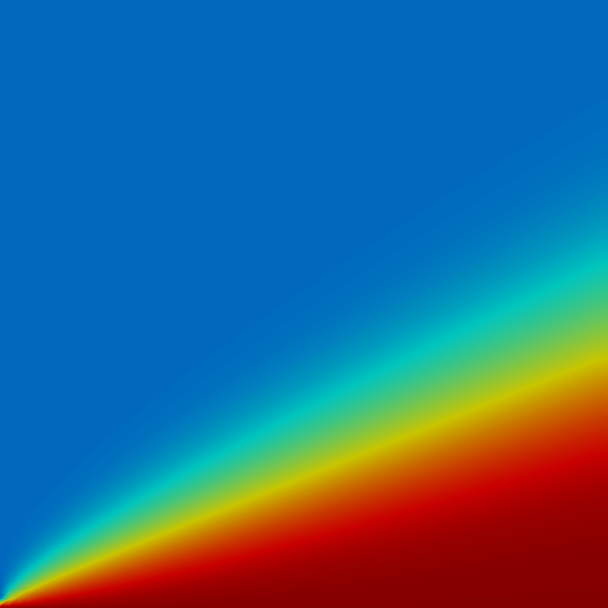
\includegraphics[width=\textwidth]
        {images/glance_Low.png}
      \caption{Low-Order}
   \end{subfigure}
   \begin{subfigure}{0.45\textwidth}
      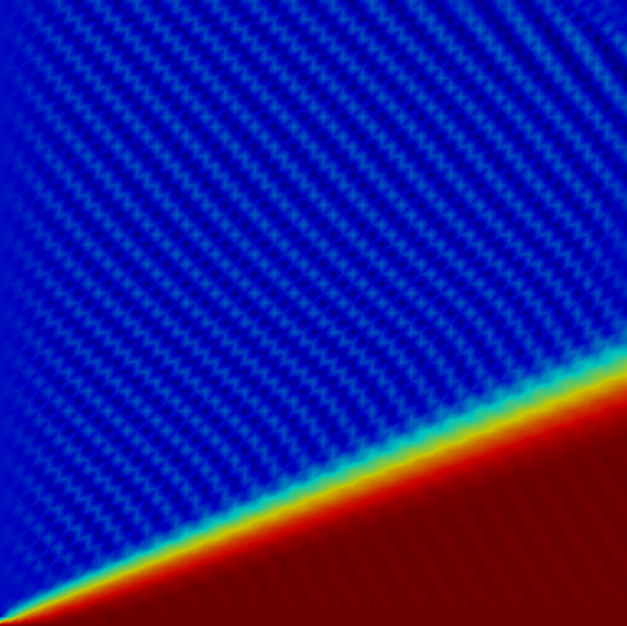
\includegraphics[width=\textwidth]
        {images/glance_EV.png}
      \caption{EV}
   \end{subfigure}
   \begin{subfigure}{0.45\textwidth}
      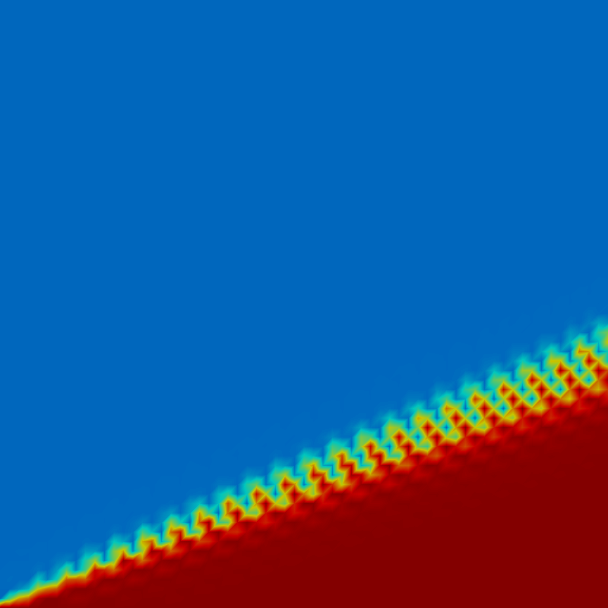
\includegraphics[width=\textwidth]
        {images/glance_GalFCT.png}
      \caption{Galerkin-FCT}
   \end{subfigure}
   \begin{subfigure}{0.45\textwidth}
      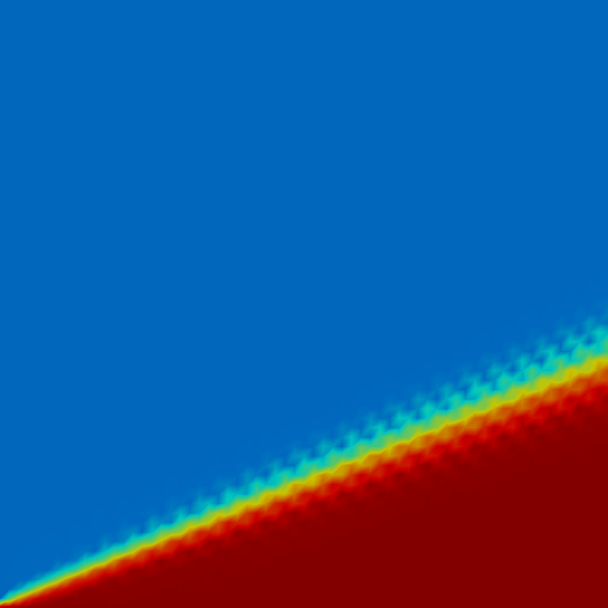
\includegraphics[width=\textwidth]
        {images/glance_EVFCT.png}
      \caption{EV-FCT}
   \end{subfigure}
   \caption{Comparison of Solutions for the Glance-in-Void Test
     Problem Using Explicit Euler Time Discretization}
   \label{fig:glance_in_void_fe}
\end{figure}
\clearpage
%===============================================================================
\subsection{Obstruction Test}\label{sec:obstruction}
%===============================================================================
This is a 2-D, two-region problem on the unit square $(0,1)^2$ with a beam incident on the
left and bottom boundaries at an angle of $45^\circ$ with the x-axis. The
center region $(\frac{1}{3},\frac{2}{3})^2$ is an absorber region
with $\sigma(\x)=10$ and $q(\x)=0$, and the surrounding region is a void
($\sigma(\x)=0$, $q(\x)=0$).

This problem was run with Implicit Euler with a CFL of 1 to steady-state on
a $32\times32$ mesh. The results are shown in Figure \ref{fig:obstruction_be}.
The low-order solution is especially diffusive and shows a fanning
of the solution after it passes the corners of the obstruction, which is
not present in any of the high-order schemes. The EV solution contains
oscillations, although they are much less significant than in the Galerkin
solution. Both FCT schemes show a lack of these oscillations, but the
Galerkin-FCT solutions shows a terracing effect. The EV-FCT solution also
has this effect but to a much smaller degree.

\begin{figure}[ht]
   \centering
   \begin{subfigure}{0.3\textwidth}
      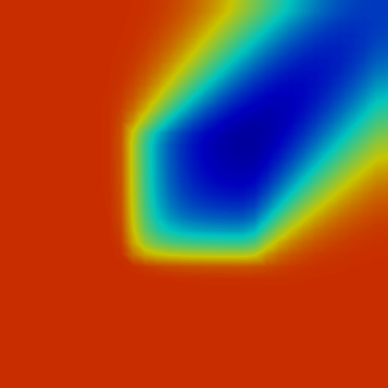
\includegraphics[width=\textwidth]
        {images/obstruction_low.png}
      \caption{Low-Order}
   \end{subfigure}
   \begin{subfigure}{0.3\textwidth}
      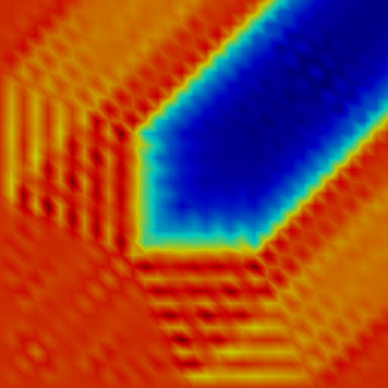
\includegraphics[width=\textwidth]
        {images/obstruction_Gal.png}
      \caption{Galerkin}
   \end{subfigure}
   \begin{subfigure}{0.3\textwidth}
      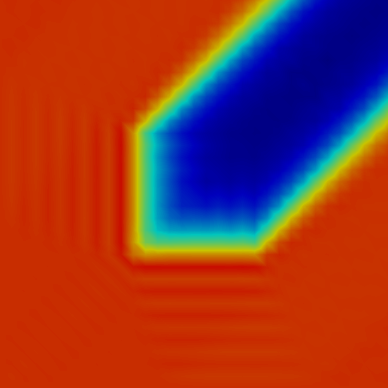
\includegraphics[width=\textwidth]
        {images/obstruction_EV.png}
      \caption{EV}
   \end{subfigure}
   \begin{subfigure}{0.3\textwidth}
      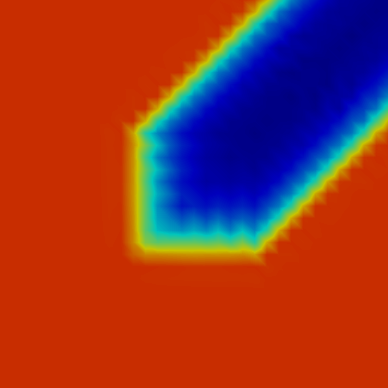
\includegraphics[width=\textwidth]
        {images/obstruction_GalFCT.png}
      \caption{Galerkin-FCT}
   \end{subfigure}
   \begin{subfigure}{0.3\textwidth}
      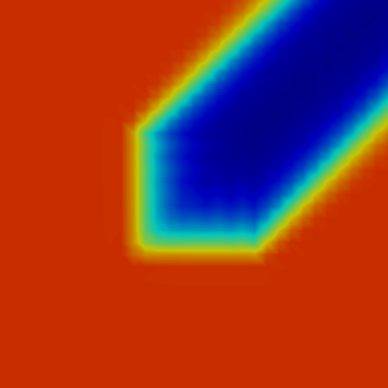
\includegraphics[width=\textwidth]
        {images/obstruction_EVFCT.png}
      \caption{EV-FCT}
   \end{subfigure}
   \caption{Comparison of Solutions for the Obstruction Test
     Problem Using Implicit Euler Time Discretization}
   \label{fig:obstruction_be}
\end{figure}

Table \ref{tab:obstruction_iterations} shows the results for a parametric study
on the number of nonlinear iterations required for EV and EV-FCT for various
CFL numbers on a $16\times 16$ mesh, to an end time of $t=1.5$. Recall that in the FCT algorithm, one first computes the high-order solution
(here, EV), which is necessary for computation of the antidiffusive fluxes.
The number of nonlinear iterations for this solve is given in the column
labeled as ``EV''. The FCT limiting procedure is also nonlinear; the number
of nonlinear iterations for this solve is given in the ``FCT'' column.
While these results indicate that increasing the CFL number decreases the total
computational work in reaching the end of the transient, it should be noted that
the quality of the FCT solution deteriorates significantly for large CFL numbers;
see the ``$L^2$ Err.'' column.
As discussed previously, the solution bounds are implicit and thus change
with each iteration. This challenge is compounded in the case of large time
step sizes; as time step size increases, the solution bounds widen, and
successive FCT solution iterates differ more than for smaller time step sizes.
This trend is suggested in the rate of increase in the number of FCT iterations per time step
in Table \ref{tab:obstruction_iterations}, which is significantly larger than the
rate of increase of EV iterations per time step. However, this issue can be mitigated
using a relaxation factor on the iterative solution updates; for example, for
the failing case of CFL number equal to 20, convergence can be achieved with a
relaxation factor of 0.9, giving average iterations per time step of
14.33 and 221.67 for EV and FCT, respectively.

%-------------------------------------------------------------------------------
\begin{table}[htb]\caption{Nonlinear Iterations vs. CFL Number for the
  Obstruction Test Problems}
\label{tab:obstruction_iterations}
\centering
\begin{tabular}{c c c c c c c}\hline
\emph{CFL} & \emph{Relax} & \multicolumn{2}{c}{\emph{EV}} & \multicolumn{2}{c}{\emph{FCT}} & $L^2$ \emph{Err.}\\
           &              & \emph{Total} & \emph{Avg.}    &  \emph{Total} & \emph{Avg.}    &\\\hline
0.1        & --  & 6204 &  8.43 & 5223 &   7.23 & $5.084\times10^{-2}$\\
0.5        & --  & 1386 &  9.36 & 2239 &  15.13 & $5.079\times 10^{-2}$\\
1.0        & --  & 791  & 10.69 & 1588 &  21.46 & $5.111\times 10^{-2}$\\
5.0        & --  & 265  & 17.67 & 1780 & 118.67 & $5.980\times 10^{-2}$\\
10.0       & --  & 150  & 18.75 & 1298 & 162.25 & $9.854\times 10^{-2}$\\
20.0       & --  & --   &    -- & \multicolumn{2}{c}{(failure)} & --\\
20.0       & 0.9 & 66   & 16.50 &  935 & 233.50 & $1.295\times 10^{-1}$\\
\hline\end{tabular}
\end{table}
%-------------------------------------------------------------------------------

\clearpage
%===============================================================================
\subsection{Two-Region Interface}
%===============================================================================
This 1-D test problem simulates the interface between two regions with
varying cross section and source values on the domain $(0,1)$.
The left half of the domain has values $\sigma(\x)=10$ and $q(\x)=10$, for which the transport
solution will reach a
saturation value of $\frac{q}{\sigma}=1$, while the right half has values
of $\sigma(\x)=40$ and $q(\x)=20$, giving it a saturation value of
$\frac{q}{\sigma}=0.5$. The transport direction is $\di=\mathbf{e}_x$, with
zero incident flux on the left boundary.

This problem was run using SSPRK33 time discretization with a CFL of 1 to
steady-state with 32 cells. Figure~\ref{fig:interface} shows the results
for this test problem. The low-order solution suffers from the significant
artificial diffusion, while the Galerkin solution suffers from significant
spurious oscillations. The EV scheme eliminates some of the first oscillations,
but a number of oscillations of a similar magnitude to those produced by
the Galerkin scheme still exists to the left of the interface.
The sets ``$U^-$'' and ``$U^+$'' correspond to the minimum and maximum solution
bounds, respectively, of each FCT scheme (the differences between the bounds of the two FCT
schemes are insignificant here).
schemes effectively eliminate spurious oscillations without approaching
the level of unnecessary artificial diffusion achieved by the low-order
scheme. For this test problem, the Galerkin-FCT solution is slightly
superior to the EV-FCT solution and the ``terracing'' phenomenon
of FCT is not present.

\begin{figure}[htb]
   \centering
      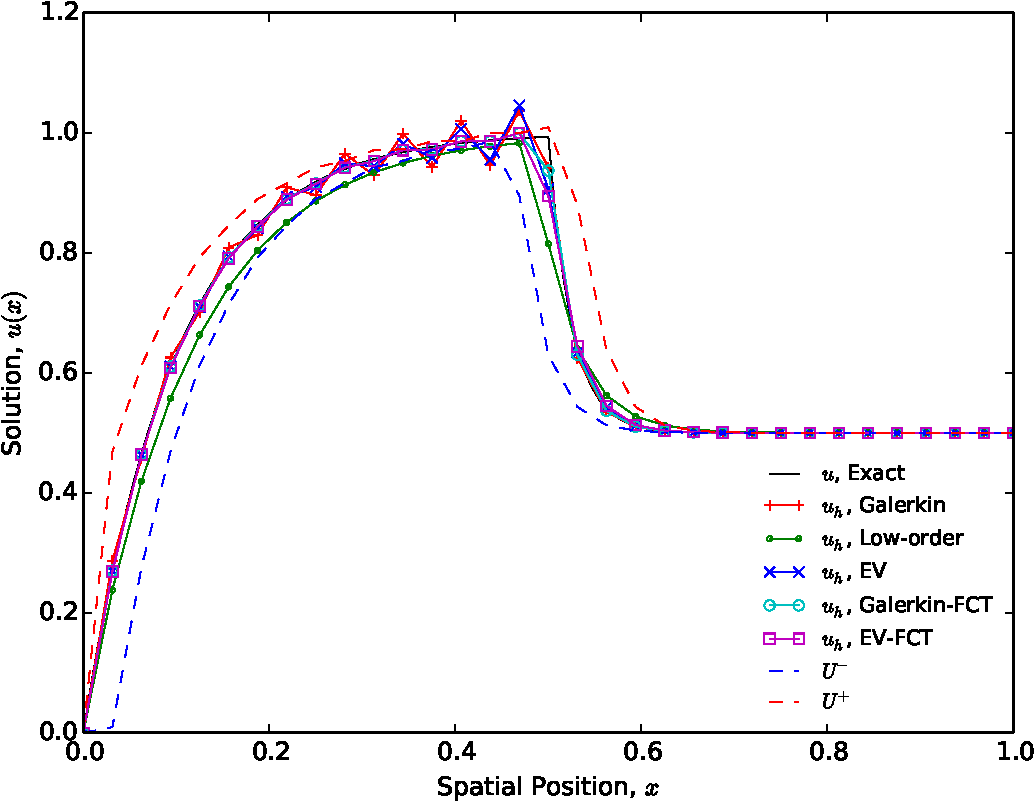
\includegraphics[width=\textwidth]
        {images/solution_interface.pdf}
      \caption{Comparison of Solutions for the Two-Region Interface Test
       Problem Using SSPRK33 Time Discretization}
   \label{fig:interface}
\end{figure}
\clearpage
%===============================================================================
\subsection{Source in a Void Test}
%===============================================================================
This 1-D test problem has two regions, the left being a void but with a source:
$\sigma(\x)=0$ and $q(\x)=1$, and the right being an absorber without a source:
$\sigma(\x)=10$ and $q(\x)=0$. This does not represent necessairly a non-physical problem:
due to the energy dependence of the particle distribution, it is possible to have
a strong inscattering source term in an energy bandwidth where the interaction coefficient is
small; here we emphasize the weak interaction probability by zero-ing out the reaction term.
A zero Dirichlet boundary condition is imposed on the incoming (left)
boundary, and this problem is run as a steady-state problem on the domain
$(0,1)$ with 32 cells.

For this problem, the entropy residual and jump coefficients $c_\mathcal{R}$
and $c_\mathcal{J}$ are set to 0.5; the default value of 0.1 was found
to be too small for this problem.
Figure~\ref{fig:source_in_void} shows the results for this problem.
The Galerkin solution has ``kinks'' along the void (left) region, but
shows point-wise matching of the exact solution in the absorber (right)
region. The EV solution, however, eliminates the terracing effect in
the void region but suffers from an inflated peak at the interface, due
to entropy production at the interface. The EV-FCT solution bounds generated for this
problem are denoted as ``$U^-$, EV-FCT'' and ``$U^+$, EV-FCT''. For this test problem, the
Galerkin-FCT scheme gives superior results to that of the EV-FCT
scheme. However, both FCT schemes suffer from the familiar FCT
phenomenon known as ``peak-clipping'', whereby the ``mass'' that
should be present in the peak has been redistributed by the FCT
limiter, flattening the peak.

\begin{figure}[htb]
   \centering
      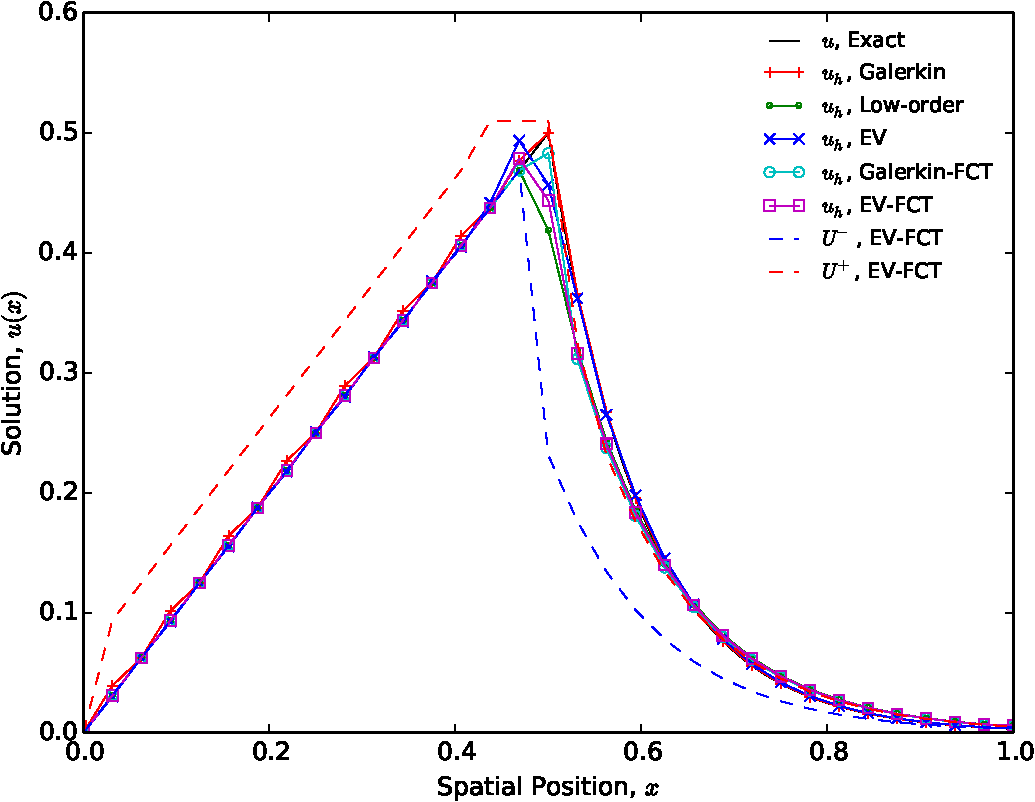
\includegraphics[width=\textwidth]
        {images/solution_source_in_void.pdf}
      \caption{Comparison of Solutions for the Source-in-Void Test
       Problem Using Steady-State Time Discretization}
   \label{fig:source_in_void}
\end{figure}
%
%For this particular test problem, the entropy viscosity method is particularly
%slow to converge its nonlinear iterations, requiring 147 iterations to
%converge, while the FCT solve took only 2 iterations. Recall that fixed-point
%iteration was used for both solves, although it isn't necessary to use a
%fixed-point method for the entropy viscosity solve; a more efficient alternative
%such as Newton's method could be used instead. The convergence difficulties
%here arise from the response of the entropy viscosity to the entropy profile
%of the previous iteration, which can create an ``entropy oscillation'' effect
%that can significantly slow convergence. However, it should be noted that the
%performance observed for this problem is not necessarily typical of all
%steady-state problems. For example, many problems do not require nearly as
%many EV iterations and require more iterations, sometimes converging as
%poorly as for the problem given in Section \ref{sec:obstruction}.

\clearpage
